% % % % % % % % % % % % % % %
\documentclass[11pt]{article}
\usepackage[a4paper, portrait, margin=1in]{geometry}
% % % % % % % % % % % % % % %

\usepackage{graphicx}
\usepackage{caption}
\usepackage{fancyhdr}
\usepackage{siunitx}
\usepackage{amsmath}
\usepackage{hyperref}
\pagestyle{fancy}
\fancyhf{}
\renewcommand{\headrulewidth}{0pt}
\renewcommand{\footrulewidth}{0pt}

\usepackage{array}
\newcolumntype{$}{>{\global\let\currentrowstyle\relax}}
\newcolumntype{^}{>{\currentrowstyle}}
\newcommand{\rowstyle}[1]{\gdef\currentrowstyle{#1}%
  #1\ignorespaces
}


\usepackage{array}
\usepackage{booktabs}

\fancypagestyle{firstpagefooter}
{
\lfoot{Version: 25.11.2016}
\cfoot{}
\rfoot{\thepage}
}
\cfoot{\thepage}


\begin{document}

\title{Advanced Systems Lab (Fall'16) -- Third Milestone}

\author{Name: \emph{Aleksander Matusiak}\\Legi number: \emph{16-931-925}}

\date{
\vspace{4cm}
\textbf{Grading} \\
\begin{tabular}{|c|c|}
\hline  \textbf{Section} & \textbf{Points} \\ 
\hline  1 &  \\ 
\hline  2 &  \\ 
\hline  3 &  \\ 
\hline  4 &  \\ 
\hline  5 &  \\ 
\hline \hline Total & \\
\hline 
\end{tabular} 
}

\maketitle
\thispagestyle{firstpagefooter}
\newpage

\iffalse
\section*{Notes on writing the report}

The report does not need to be extensive but it must be concise, complete, and correct. Conciseness is important  in  terms  of  content  and explanations,  focusing  on  what  has  been  done and  explanations  of the results. A long report is not necessarily a better report, especially if there are aspects that  remain  unexplained.  Completeness  implies  that  the  report  should  give  a comprehensive idea of what has been done by mentioning all key aspects of the modeling and analysis effort. Limited analysis because of flaws in the system or lack of experimental data from Milestones 1 or 2 are not  valid  arguments  for  an incomplete  report.  If  bugs  or  lack  of  data  prevent  you  from  doing  a  correct analysis, the system must be debugged and new data collected. In case the system has been modified, include a short description of the changes as an appendix.

Remember  that  this is  a  report  about modeling  and  analyzing the  system you  have  designed  and  built, using  the experimental data you have collected. There is no unique way to do the report and you may choose  to  focus  on  different  aspects  of  the  system  as  long  as  you deliver a  complete analysis of  its behavior. Keep in mind that, \emph{for all queuing models in the report}, you need to explain how the the parameters of the model were determined and from which experiments the data comes from (adding a reference to the exact graph, table, etc. from the previous milestones). You have to find all system metrics that can be derived using the corresponding formulas and then match to the experimental results, explaining the similarities and differences in quantitative and qualitative terms. The calculations and the numbers you derive might need to be explained with references to the logs and sources in the previous reports. Make sure to mark these references, as well as the ones pointing to experimental results clearly. \textit{Missing parts of the above requirements might lead to significant loss of points in each section.}

The report should be organized in sections as explained in the next pages, and each section should address at least the questions mentioned for each point. You might be called for a meeting in person to clarify aspects of the report or the system and to make a short presentation of the work done. By submitting the report, you  confirm  that  you  have  done  the  work  on  your  own,  the  data used comes  from  experiments  your have  done,  you  have  written  the  report  on  your  own,  and  you have  not  copied  neither text nor data from other sources.

\medskip
The milestone is worth 200 points. 


\pagebreak
\fi

\section{System as One Unit}\label{sec:system-one-unit}

\iffalse
Length: 1-2 pages

Build an M/M/1 model of your entire system based on the stability trace that you had to run for the first milestone. Explain the characteristics and behavior of the model built, and compare it with the experimental data (collected both outside and inside the middleware). Analyze the modeled and real-life behavior of the system (explain the similarities, the differences, and map them to aspects of the design or the experiments). Make sure to follow the model-related guidelines described in the Notes!
\fi


In M/M/1 model we have one queue and one server. As server we will consider memcached server. Since there are actually 3 memcached servers processing requests, we will have to calculate the service rate accordingly. We do not consider clients as a part of our system - as the system we take our middleware and connected memcached servers.

%For this model we take server discipline First Come First Served, with no buffer limitations. 
The population size is 192 clients and the system is a closed one. All values have been calculated based on formulas in Box 31.1 from the course book.

In order to provide more detailed analysis I have enhanced logging inside the middleware (see the appendix for detailed changes). Therefore I had to rerun the stability trace (plots provided in the appendix) as well as other experiments, from which data is used in the next sections. Logs for the repeated stability trace are in files: mm1\_1, mm1\_2, mm1\_3, mm1\_parsed (see appendix for links). I run the new experiment for 30 minutes (which was enough to prove that the system was stable and to gather appropriate data).

Throughput measured by memaslap clients was equal to 13758 operations/second. Therefore, I take arrival rate $\lambda = 13758 \textrm{ ops/s}$. One approach to calculate the service rate is to take maximum throughput measured during the experiment. This approach has been suggested during the tutorial and gives us a lower bound on a service rate. This is because if system was able at some point in time to have this performance, it means that it is able to perform at least that well. Since the running time of the experiment was pretty long (30 minutes), we can assume that this approximation is good enough.

Another approach to do this would be to calculate the number of requests being actively processed in the middleware, which corresponds to the average parallelism in the middleware. We would then assume that the service time is average time spent in the servers divided by the number of active threads. We still would need to take into the account that this time includes requests being sent over the network, but we could also treat network as a queue. Since servers have only 1 thread working the requests will partially wait in the queue of the server and partially this waiting period will be included in the time spent in the network. However, this approach proved to be inaccurate. For this task I got the following results: on average 38.15 getter threads are busy processing requests and there are on average 1.05 requests in all setter threads (there are 3 of them). So, on average, there are $m = 39.21$ on the fly (sum based on more precise numbers). That would mean service rate approximately 13893 requests/second and would result in a very high utilization - around 99\%. For the second task, however, utilization calculated using this approach was over 1. This is because in order to use this method we have to assume that memcached servers are busy almost all the time and time spent in the network, even without network, would be spent in the queue. However, this is not the case and therefore results of this method are unsatisfactory. 

%I had to improve the logging in my middleware (see apendix) in order to log also current numbers of busy getter threads and number of requests processed currently by setter requests (i.e. number of set requests that have been taken out of the queue but the response for them has not yet been sent to the client). This made it necessary to repeat the experiment.

%Looking at the middleware logs I have calculated, that an average time spent in the servers equals: $T_s = \SI{2841.63}{\micro\second}$, which is the difference between $T\_SendToClient$ and $T\_Dequeue$ (see report for milestone 1.). When it comes to number of requests on the fly I got the following results: on average 38.15 getter threads are busy processing requests and there are on average 1.05 requests in all setter threads (there are 3 of them). So, on average, there are $m = 39.21$ on the fly (sum based on more precise numbers). Based on the previous analysis we can now calculate the service rate appropriate for M/M/1 model:

Looking at the memaslap logs I have calculated that maximum throughput was equal to 16701 requests/second. Therefore, using the first described approach, we have:
$\mu = 16701\textrm{ req/s}$.
%$$\mu \approx \frac{39.21}{2841.63} \cdot 10^6 \textrm{ requests/second} \approx 13892.53 \textrm{ requests/second}$$
%In order to calculate mean service rate which includes that many requests are processed in parallel, I had to find out the average number of requests being in the service. In order to do that I had to make some changes in my code (described in the appendix) i I 
This enables us to calculate the offered load:
$\rho \approx 82.38\%$.
The offered load is below 1, which means that the system is stable. It means that $82.38\%$ of the time the server is busy.
%The utilization can be considered to be pretty high. It stems from the fact that for stability experiment I have used only 16 threads. As the experiments from second milestones have shown, for 16 threads we get worse performance than for the higher number of threads. This means that threads are mostly busy and since the high utilization of the system. What is more, the component that causes this high utilization is accepting thread. As I have pointed out in the report for milestone 2, this component at some point becomes the bottleneck of the system. For stability trace It was still not the case (too low number of threads), but this component either way is not that effective and affects the offered load.
Consequently we get that the  probability that there are zero jobs in the system equal: $1 - \rho \approx 17.62\%$. 
This result is not consistent with the data collected from the middleware. We can calculate that the first percentile of number of active getter threads is already equal 8. This means that 99\% of the time they are not less than 8 get requests being processed in the system. This contradicts result from the theory. This can be explained in a following way: M/M/1 models do not take into the account the possibility that several requests can be processed at the same time. Based on the high service rate from model we get that the single request is processed really quickly, so that they don't queue that much. However, in reality, requests are processed for a longer time, but they are several requests processed in parallel. In a similar way, when we calculate the average number of requests in the system, we get contradicting results. We have:
$E[n] 
%=\frac{\rho}{1 - \rho} \approx{82.38\%}/{17.62\%} 
\approx 4.67$.
We know from the collected logs that on average there are around 39 requests being processed at the same time. This means that they are at least 39 requests in the whole system. The reason for this discrepancy is the same as mentioned above - M/M/1 model does not consider the parallelism. Variance for $n$ was calculated to be around $26.5$, measured value was equal around $118.5$, which is around $4.5$ times higher. This suggests that the number of jobs in our system was, proportionally, less varied - difference in variance is way smaller than squared difference for mean value.

% Remove if not enough space
%It is also worth pointing out here, that measured average number of set requests being serviced is quite low, considering that there are 3 setter threads (one for each queue) which process requests asynchronously (one thread can process more than one requests at the same time). This is because set requests are only 1\% of all requests, so they are not many of them and although it takes longer to process them, the low number of them leads to low number of them being processed at the same time.

When we take a look at calculated mean number of jobs in the queue and in the service we still see discrepancies, but there is one thing that is similar to measured values:
$E[n_q] 
%= \frac{\rho^2}{1-\rho} 
\approx 3.85$ and
$E[n_s] 
%= \rho 
\approx 0.82$.
The ratio of jobs in the queue to jobs in the system is equal to $\rho \approx 0.823$ (simple formulas transformation). Under the assumption that almost all of 192 requests are in the system, we have that around 39 requests are being processed (see earlier) and therefore $192-39 = 153$ jobs are in the queue. The ratio between jobs in the queue and jobs in the system equals here to $\frac{153}{192} \approx 0.797$. These values are relatively close to each other, so we can say that this ration has been well predicted by our model. Variance for $n_q$ was calculated to equal around $25.0$ - we cannot, however, compare this with measured data, since we didn't provide appropriate logging facilities for that (we're not counting number of requests in the queue). 

%The probability that there are $n$ jobs in the system equals approximately $p_n = 0.97\% \cdot 99.03\%^n$. We can also calculate how many requests are in system in total:
%$$E[n] = \frac{\rho}{1 - \rho} \approx{99.03\%}/{0.98\%} \approx 102.52$$
%Let me remind here that there are 192 clients. Calculated number is therefore plausible. Requests spend also significant amount of time traveling in the network between memaslap clients and middleware, which causes the calculated number of requests in the system to be a lot less than the number of clients.

We can calculate also mean response time:
$E[r] 
%= (1/\mu)/(1 - \rho) \approx \frac{1}{16701 \textrm{ requests/second} \cdot 17.62\%} 
\approx \SI{339.82}{\micro\second}$.
When we look at the data collected from the middleware we can see that the mean time spent in the middleware equals approximately \SI{7655}{\micro\second} (we take time spent inside the middleware cause it better corresponds to the calculated response time than response time measured by clients, which include also additional network time). This does not correspond at all to the calculated mean response time. This can again be explained by the fact that our model is not appropriate for handling parallelism. High service rate means, for M/M/1 model, that the requests are processed quickly and do not spend much time in service and, in consequence, in the middleware. In reality it takes some time to process the request, which results in way higher measured time spent in the middleware. The same applies for mean waiting time (time in the queue) and mean service time. From theory we have:
$E[w] 
%= \rho \frac{1/\mu}{1 - \rho} \approx 82.38\% \cdot \frac{1/16701}{17.62\%} 
\approx \SI{279.95}{\micro\second}$ and
$E[s] 
%= \frac{1}{\mu} 
\approx \SI{59.88}{\micro\second}$.
The corresponding values measured by the middleware equal: \SI{3203}{\micro\second} for time spent in the queue (which is part of the system representation) and \SI{2841}{\micro\second} for the time spend in the servers. We can see that measured time spent in the servers is approximately 47 times higher then calculated service time. This value is comparable to 39 requests on the fly (mentioned earlier), but it better corresponds to the parallelism of the middleware, since it also reflects the fact that servers do not have to be busy all the time. Below we present some more statistics:
%Let's not forget here that requests also spend some time waiting for the accepting thread to be parsed, so that the difference between waiting time predicted and measured is even higher.

{\small
\begin{center}
\begin{tabular}{|c|c|c|c|c|}
\hline & $Var[r]$ ($\SI{}{\micro\second}^2$) & 90-th perc. $r$ ($\SI{}{\micro\second}$) & Var[w] ($\SI{}{\micro\second}^2$) & 90-th perc. $w$ ($\SI{}{\micro\second}^2$)\\
\hline Calculated & 115482 & 781 & 111896 & 717\\
\hline Measured & 180146340 & 13993 & 117574816 & 10476 \\
\hline Ratio & 1560 &  17.9 & 1051 & 14.6\\
\hline
\end{tabular}
\end{center}
}
We can clearly see that measured statistics are much higher, because of the parallelism and the fact that corresponding mean values are also higher. Bigger difference in variance is because when calculating variance we are dealing with squares, so the values are also bigger (and so is the ratio). However, the ratio (or root of the ration for variance) is smaller than parallelism calculated based on mean response times values (around 47), which again suggests that the real behavior of our system is less varied. This can be explained by the fact that real implementation of the system is much more complex than the model we are using. Different factors inside the middleware are connected with each other and cooperation of different components lowers the variation of data. What is more, the distribution of the arrival rate might be different than the one that M/M/1 model assumes (Poisson distribution). 

\iffalse
Another statistics calculated based on the model, but not comparable to the measured values (not enough measured data) are as follows:

{\small
\begin{center}
\begin{tabular}{|c|c|}
\hline Mean number of jobs served in one busy period & 5.7 \\
\hline Variance of number of jobs served in one busy period & 274.7 \\
\hline Mean busy period duration & \SI{340}{\micro\second} \\
\hline Variance of the busy period & $\SI{539929}{\micro\second}^2$ \\
\hline
\end{tabular}
\end{center}
}
\fi

To sum up, M/M/1 model does not reflect our middleware properly. It does not take into the account the parallelism and predicted values differ significantly.

%$$E[r] = \frac{1/\mu^2}{(1 - \rho)^2} \approx \frac{1/13893^2}{0.97\%^2}$$
%The 90th percentile calculated equals to : $2.3 E[r] \approx \SI{17138}{\micro\second}$. When we look at the data from middleware we can see that 90th percentile actually equals around \SI{13880}{\micro\second}, which is lower than the time calculated from the model.
% TODO: explain

%We can also calculate the time spent in the queue:
%$$E[w] = \rho \frac{1/\mu}{1 - \rho} \approx 99.03\% \cdot \frac{1/13893}{0.97\%} \approx \SI{7379}{\micro\second}$$
%Mean time spent in the queue (being part of the implementation) measured by the middleware is around \SI{4768}{\micro\second}. The differences here are much more significant then overall response time. This is because the queue from the implementation does not correspond to the queue in the M/M/1 model. Requests have to wait also in the queue for each server and also spend some time in the network (which can be treated as a part of the queue, as explained above). What is more, since we have 3 servers, more requests than 1 can be processed by them in parallel, which means that the time spent in the queue measured will be even lower than this calculated.

%When we look at the data collected from the middleware we can see that the mean time spent in the queue (being part of the implementations) is equal to around \SI{3203}{\micro\second}. The difference between this values stems from the fact that in our model we have one queue, which includes also waiting by the request to be handled by the thread handling network messages. As described in the report for milestone 2., this point of the system becomes at some point the bottleneck, so it's reasonable that waiting time here is also significant.

\clearpage

\section{Analysis of System Based on Scalability Data}\label{sec:analysis-scalability}

\iffalse
Length: 1-4 pages

Starting from the different configurations that you used in the second milestone, build M/M/m queuing models of the system as a whole. Detail the characteristics of these series of models and compare them with experimental data. The goal is the analysis of the model and the real scalability of the system (explain the similarities, the differences, and map them to aspects of the design or the experiments). Make sure to follow the model-related guidelines described in the Notes!
\fi

In this section we will model a system as a queue with $m$ servers processing the requests. The system under test is going to be defined as our middleware together with memcached servers. We will take $m$ equal to the number of memcached servers used for the given experiment and in our model each server will correspond to threads associated with one queue forwarding request together with the according memcached server. As it will be pointed out, this model won't correspond properly to the behavior of the system, since each server can in fact process more than 1 request at the same time (which is the underlying assumption for the model). I have decided for this model because the number of resources (servers) here corresponds to the actual number of core functionality resources (memcached servers; middleware is only for forwarding requests, not actually providing core functionality of the whole system). Since I include the processing threads as a part of the service, I don't have to change the arrival rate to include increased number of requests sent to the memcached servers because of the replication. Actual number of requests that arrive to the threads is the same as number of requests sent to the clients and replication will be included in the service time.

%For this model we take server discipline First Come First Served, with no buffer limitations.
The population size is 210 clients. To create models for this section I have used the approach presented in the section \ref{sec:system-one-unit}, which is calculating service rate based on the maximum throughput. In the experiments described in this section runtime was shorter than in the stability experiment, but still we collected 180 values for the throughput (measuring every second for one minute, 3 replications). This enabled us to, once again, achieve quite good approximation. Another approach (dividing server time by the number of requests on the fly) would result in utilization over 1.

\iffalse
In the scalability experiments analysis we also have to account for the fact that having replication increases load on the servers. Let us then introduce following symbols for parameters and measured values: $T$ - measured mean throughput, $M$ - measured maximum throughput, $w$ - writes percentage, $r$ - numbers of servers to which we replicate, $m$ - number of servers. Lets also take $N$ as the number of requests send by the clients to the middleware. Distinguishing between get and set requests, we have that all servers have to process $N'$ requests, where:
$$N' = N (1 - w) + wrN = N (1 + w(r - 1))$$
When we aggregate number of requests during one second and take an average, we can calculate the mean arrival rate:
$$\lambda = T (1 + w(r - 1))$$
When we want to calculate now the service rate based on the maximum throughput, we also need to include this factor. This is because we're actually counting the number of requests being processed by the middleware at the peak performance, so if we modify the number of requests that arrive to the system, we also need to modify the number of requests that get out of the system accordingly. Therefore, when we include that there are $m$ servers processing requests from one queue, we have:
$$\mu = \frac{M  (1 + w(r - 1))}{m}$$

When we now calculate the traffic intensity, introduced additional factors which account for replication, are reduced:
$$\rho = \frac{\lambda}{m \mu} = \frac{T}{M}$$
\fi

There have been many different configurations used in the scalability experiments from previous milestone (task 2. and 3.). In order to provide a detailed analysis of created models I have focused my attention on creating models for extreme configurations - 3 and 7 servers, no replication and full replication, 1\% and 10\% of write requests. This will result in creating 8 models. We want to analyze the scalability of our system so I will look into increasing number of servers under 4 configurations (possible configurations for extreme values of replication factor and writes percentage; effect of these factors on performance will be analyzed in section \ref{sec:2k-experiment}). All of these configurations have been investigated for task 3. from previous milestone.

In order to provide a proper analysis of the model, I had rerun the experiments from milestone 2. task 3. (results from this task I'm using in this section). I have used the same configuration as provided in the section 3.2 of my report from the previous milestone. The only difference was in the logging facilities introduced for the middleware (for changes in the source code - see appendix). The new log files have corresponding names to those used in the previous milestones, but have 'improved-' prefix (for log files list - see appendix).


\subsection{Input data for models}

In the table \ref{fig:input} is presented the necessary data to create before mentioned models. I have calculated $\mu$ based on above formula.

\begin{figure}
{\small
\begin{center}
\begin{tabular}{|$c|^c|^c|^c|^c|^c|^c|^c|}
\hline
\rowstyle{\bfseries} 
$m$	& Rep.	&	 \parbox[t]{2cm}{Writes percentage (\%)} &	T	&	$\lambda$	&	M	&	$\mu$	 \\

\hline 3 & none & 1 & 15687 & 15687 & 19860 & 6620 \\ 
\hline 7 & none & 1 & 12730 & 12730 & 16187 & 2312 \\ 
\hline 3 & all & 1 & 15556 & 15556 & 19590 & 6530 \\ 
\hline 7 & all & 1 & 12070 & 12070 & 14769 & 2110 \\ 
\hline 3 & none & 10 & 15340 & 15340 & 19227 & 6409 \\ 
\hline 7 & none & 10 & 12547 & 12547 & 15954 & 2279 \\ 
\hline 3 & all & 10 & 14353 & 14353 & 17807 & 5936 \\ 
\hline 7 & all & 10 & 10139 & 10139 & 13592 & 1942 \\ 
\hline
\end{tabular}
\end{center}
}
\caption{Input data}
\label{fig:input}
\end{figure}

Let us point out here that $\mu$ (for each server) is significantly decreasing as we increase the number of servers. This should not be the case according to the theory - $\mu$ should be the same for each server, independently on their number and increasing number of servers should only increase the effective service rate ($m\mu$). However, in theory increasing number of servers means increasing number of resources available. We increase the number of resources available for memcached servers, but the number of resources available on the side of middleware stay the same (we have only 8 cores), what is more, with more servers we have more threads, which even more decreases the performance and results in decreased $\mu$.

\subsection{Number of requests}

Based on this data we can compute system properties. I have used formulas from Box 31.2 in the course book.

Let us define: $P_0$ - probability that there are 0 jobs in the system, $P_q$ - probability of queuing, $R_g$, $R_s$, $R$ - number of, respectively, get, set and all requests on the fly. Rep. is an abbreviation for replication factor and W. - for percentage of write requests. Other definitions are the same as in the book.

{\small
\begin{center}
\begin{tabular}{|$c|^c|^c|^c|^c|^c|^c|^c|^c|^c|^c|^c|^c|}
\hline
\rowstyle{\bfseries} 
$m$	& Rep.	&	W. & $\rho$ & $P_0$ &	$P_q$	&	$E[n]$ 	&	$E[n_q]$	& $E[n_s]$ &	$R_g$ & $R_s$ & $R$ & $\frac{R}{E[n_s]}$  \\
\hline 3 & none & 1 & 0.790 & 0.060 & 0.631 & 4.74 & 2.37 & 2.37 & 52.06 & 1.21 & 53.27 & 22.48 \\ 
\hline 7 & none & 1 & 0.786 & 0.003 & 0.458 & 7.19 & 1.69 & 5.51 & 72.87 & 1.17 & 74.03 & 13.45 \\ 
\hline 3 & all & 1 & 0.794 & 0.058 & 0.638 & 4.84 & 2.46 & 2.38 & 54.66 & 1.25 & 55.91 & 23.47 \\ 
\hline 7 & all & 1 & 0.817 & 0.002 & 0.523 & 8.06 & 2.34 & 5.72 & 71.91 & 1.26 & 73.17 & 12.79 \\ 
\hline 3 & none & 10 & 0.798 & 0.057 & 0.644 & 4.93 & 2.54 & 2.39 & 48.89 & 12.48 & 61.37 & 25.64 \\ 
\hline 7 & none & 10 & 0.786 & 0.003 & 0.458 & 7.19 & 1.69 & 5.50 & 65.90 & 11.91 & 77.82 & 14.14 \\ 
\hline 3 & all & 10 & 0.806 & 0.054 & 0.657 & 5.15 & 2.73 & 2.42 & 48.02 & 13.23 & 61.25 & 25.33 \\ 
\hline 7 & all & 10 & 0.746 & 0.005 & 0.380 & 6.34 & 1.11 & 5.22 & 67.63 & 12.78 & 80.41 & 15.40 \\ 

\hline
\end{tabular}
\end{center}
}

From above table we can see that traffic intensity (utilization) for each server does not differ much as we increase number of servers and vary the configuration. The most significant difference can be seen for configuration (all, 10) (first element - describes replication factor, second - writes percentage). There increasing number of servers result in decrease in traffic intensity of around 0.06. In theory, 
%traffic intensity should decrease as we increase number of servers - we should be able to achieve higher service rate, since service rate for each server should be independent and increasing their number should increase the effective service rate. 
with more servers load for each servers should also decrease, so it should result in the decrease in the traffic density. However, the bottleneck of the whole system is middleware, not memcached servers, which is not well illustrated by our model. This means that as we increase number of servers load on the middleware is not decreasing and therefore traffic intensity does not change that much. It must be pointed out here that average utilization of each server is equal to traffic intensity. 

As we increase the number of servers, $P_0$ value significantly decreases. This is understandable, since for 7 servers we get worse performance (as analyzed in the report for milestone 2.), so most of the time some requests will be in the middleware.
The probability of queueing is also decreasing as we increase the number of servers. This corresponds to our system design - with more servers we have more threads which take requests from the queue. Although altogether they might not be processed faster, workers can take them out of the queue more effectively. Even when the worker after it takes out the request from the queue looses it's processing time (becomes idle), the request is already being considered as being processed. 

From above table we can also see that the calculated number of requests in service does not correspond at all to the number of requests on the fly. The actual number of requests on the fly is always at least 13 times higher than the calculated value. 
This is because our model does not take into the account the parallelization gained from dozens of threads sending the requests to the memcached servers. In M/M/m model we can have only maximally $m$ jobs being processed at the same time. However, our middleware was able to process 90 get requests (for 3 servers) and 210 get requests (for 7 servers) in parallel, as well as theoretically unbounded number of set requests. This is why these values differ so much. When we calculate the ratio of number of measured requests on the fly and calculated number of requests in service as we increase the number of servers we can clearly see that it is decreasing around 1.6 - 1.9 times. This is because we have only limited number of cores available for our middleware. When increasing number of servers we also increase the number of processing threads. Since there are only 8 cores, more threads mean less CPU time for each thread. The threads cannot perform there that well and less of them are used (some of them may not even at all be granted some CPU time). Therefore with increase of servers we notice less increase in the measured number of requests on the fly than for the calculated value (which does not represent well limited number of cores). 

%With introducing middleware we add overhead to processing the request and increase the response time (comparing to the case when we send requests directly to the memcached servers). 
 
I have not collected measured data for number of requests in the queue. It would also significantly differ from above calculations and one could expect that the ratio would be similar to the ratio already calculated.

Worth pointing out is the fact that, according to the model, when we increase the number of servers, the number of requests in service is increasing, while number of requests in the queue is decreasing. This is understandable - with more servers more requests can be processed at the same time. Whet it comes to number of requests in the queue, with the same number of clients we have more processing elements, so lower number of requests would have to be queued.

%As we increase number of servers we can clearly see the increase in the number of get requests in the server. This corresponds well to the design of our system - increasing number of servers means increase in the number of getter threads processing requests. So more requests can be processed at the same time. We can also actually see the increase in the number 

It is worth noticing here that problems with huge differences between calculated number of requests and measured is similar to the case with M/M/1 model. Here we account for a little more parallelization than in the previous section, but we still don't consider many requests being processed in parallel for one server inside the middleware. One could try to take as an a number of servers the total number of threads in thread pools or the number of requests on the fly. However, this would not correspond to processing of the set requests - they are processed in the different way inside our middleware. Therefore that model might also not fit properly our system. Only network of queues described in the section \ref{sec:network-of-queues} could account for the whole parallelism available in our system (but it will still not correspond well to the real-word situation with limited number of cores).

% TODO: add variance

%TODO: have I mentioned decrease in ratio of active threads???

\subsection{Response times and times breakdown}

Let us define: 
%$T$ - mean response time measured by the memaslap clients, 
$T_r$ - time spent in the middleware, $T_w$ - time spent in the queue, $T_s$ - time spent in the servers. 

%TODO: maybe add response time from clients ...
% TODO: make it fit
{\small
\begin{center}
\begin{tabular}{|$c|^c|^c|^c|^c|^c|^c|^c|^c|^c|^c|^c|^c|^c|}
\hline
\rowstyle{\bfseries} 
$m$	& Rep. & W.  & $E[r]$ & $E[w]$ & $E[s]$ & $T_r$ & $T_w$ & $T_s$ & $\frac{T_w}{E[w]}$ & $\frac{T_s}{E[s]}$  & $\frac{R}{m}$ & $\frac{E[s]}{E[w]}$ & $\frac{T_s}{T_w}$  \\
\hline 3 & none & 1 & 302 & 151 & 151 & 6005 & 2551 & 3419 & 16.88 & 22.63 & 17.76 & 1.00 & 1.34 \\ 
\hline 7 & none & 1 & 565 & 132 & 432 & 8818 & 3056 & 5698 & 23.07 & 13.18 & 10.58 & 3.26 & 1.86 \\ 
\hline 3 & all & 1 & 311 & 158 & 153 & 6342 & 2706 & 3592 & 17.13 & 23.46 & 18.64 & 0.97 & 1.33 \\ 
\hline 7 & all & 1 & 668 & 194 & 474 & 9370 & 3226 & 6089 & 16.66 & 12.85 & 10.45 & 2.45 & 1.89 \\ 
\hline 3 & none & 10 & 322 & 166 & 156 & 6770 & 2511 & 4217 & 15.16 & 27.03 & 20.46 & 0.94 & 1.68 \\ 
\hline 7 & none & 10 & 573 & 134 & 439 & 9342 & 3124 & 6135 & 23.25 & 13.98 & 11.12 & 3.26 & 1.96 \\ 
\hline 3 & all & 10 & 359 & 190 & 168 & 6836 & 2400 & 4389 & 12.62 & 26.05 & 20.42 & 0.89 & 1.83 \\ 
\hline 7 & all & 10 & 625 & 110 & 515 & 11554 & 3526 & 7951 & 32.07 & 15.44 & 11.49 & 4.68 & 2.25 \\ 
\hline
\end{tabular}
\end{center}
}

I will compare times from the solution of the model to times measured by the middleware. I am not focusing my attention on response time from memaslap logs, since clients are not part of my system (according to my definition) and the actual response time of the system should correspond to the time spent in the middleware.

When we compare measured times with times calculated by the model we can, once again, see huge discrepancies. Times calculated by the model are many times lower than these measured. This can again be explained by not taking the whole parallelization into the account when constructing the model. In order to account to the same effective service rate as measured, our 3 and 7 servers have to process the requests very quickly. In the real system processing the requests does not have to be very fast, because we can process many requests in parallel and each of this processing can take longer time. As we decrease the parallelism (when going from our implementation to the model), in order to keep the same service rate, response time has to decrease accordingly.

The ration between corresponding times are, however, more or less similar to the number of requests on the fly per each memcached server. This is because $\frac{R}{m}$ factor is the parallelism factor that our model is missing. We can clearly see that ratio of service time and servers time is always greater than corresponding number of active threads. This corresponds to the results I already mention in the section \ref{sec:system-one-unit}. This can be explained by the fact that memcached servers are not the bottleneck of the system. If ratio of service to servers time would be similar to number of requests on the fly, it would mean that memcached servers are almost all the time busy and time spent in the network would otherwise be spent in the queue of the memcached server. This is not the case, so servers time measured must be higher than $E[s]\frac{R}{m}$ - some of this time is also spent in the network while memcached servers are idle and waiting for new requests.

We can also see clearly see that ratio of measured and calculated waiting time is smaller than ratio of measured and calculated service (servers) time for $m=3$ and greater for $m=7$. This is because as we increase the number of servers, the ratio for service time is decreasing, also like number of requests on the fly per server. Number of requests on the fly per server decreases, because with more threads we have more operating system and context switching overhead and our threads cannot be that effective and therefore lower number of them is used. On the other hand, ratio for waiting time is almost always increasing (when we go from 3 to 7 servers; apart from (all, 1) configuration). This is because with more servers waiting time predicted by the model usually decreases (since we have lower number of requests per server), but measured time spent in the queue always increases (because of more overhead connected with increase in the number of threads).

As we increase number of servers, the ratio of service time to waiting time increases, both for calculated and measured values. This is because time spent in the servers is increasing, but calculated waiting time usually decreases and measured waiting time increases slower (the increase in the waiting time is connected with the overhead on the middleware, increase in the waiting time is also connected with establishing more network connections and overhead of the network).

%As we increase replication factor and writes percentage (together or separately) the ratio between expected service time and expected waiting time is usually decreasing (apart from one case, when it doesn't change significantly). 

\subsection{Conclusions}
As I have shown in my analysis, M/M/m model does not correspond well to the implemented system and do not account for the whole parallelization of the system. As we scale our system (increase the number of servers), the model starts to better approximate the real behavior of the system. This is because we increase the parallelism of the model, we also increase the parallelism for our implementation, but the limitation in the number of cores prevent us to increase this parallelism as much as we would like to (if we wanted to maximize the performance of our middleware).

It is also worth pointing out here that we have created models that combine set and get. Both of these type of requests have different statistics and are processed in the different way. However, such simple model as M/M/m would be unable to include these different ways of processing requests. A proper distinction between these types will be introduced in the next section.

\clearpage

\section{System as Network of Queues}\label{sec:network-of-queues}

\iffalse
Length: 1-3 pages

Based on the outcome of the different modeling efforts from the previous sections, build a comprehensive network of queues model for the whole system. Compare it with experimental data and use the methods discussed in the lecture and the book to provide an in-depth analysis of the behavior. This includes the identification and analysis of bottlenecks in your system. Make sure to follow the model-related guidelines described in the Notes!
\fi
%In order to reflect the whole parallelism available in the middleware it's necessary to expose all the components that can process the requests in parallel. For these purpose network of queues fits quite well.

In this section I have analyzed the behavior of the system under extreme conditions - 7 servers, replication to all servers and 10\% of writes. In order to analyze the network I have used Mean Value Analysis presented in Chapter 36. of the book. In order to run an appropriate algorithm to solve the model I have used Java Modelling Tools\footnote{\url{http://jmt.sourceforge.net}}, more precisely its JMVA module. It enabled me to achieve carefully calculated statics of my system. For load dependent devices this tool, however, does not support multiple classes (get and set requests). Therefore I had to provide this tool with 2 different models, which will correspond to sub-models of my queueing network model corresponding to 2 types of requests.

% \subsection{General model description}

I have created a closed queueing network, which means that the clients are also a part of the system. This enabled me to use MVA technique presented in Chapter 36. I have modeled clients and traveling of requests through the network between clients and the middleware as a delay center with service time equal to difference in mean response time measured by memaslap clients and mean time spent in the middleware. Therefore, I take $Z=0$ as a think time for clients (JMT does not allow to input this time). In my model there is one accepting thread which takes the requests from the clients and distributes them between the queues for get and sets assigned to each memcached server. 
Queues for getter and setter workers will enclose appropriate processing by memcached servers. Reasons for that are explained in section \ref{sec:bottleneck}.

\subsection{Get requests sub-model}

For this sub-model I have used 189 clients (on average 90\% clients out of 210 send get requests). I model getter worker as M/M/30 queue - they are 30 threads ready to process the request. They are 7 such queues and for each of them we have number of visits to it equal $\frac{1}{7}$ (1 in 7 requests visits this device).
% TODO: maybe some more explanation for that. 
Based on the middleware logs I take service time for accepting thread equal to \SI{31}{\micro\second}.
Since I model get queues as M/M/30 model, I have to consider these devices as load dependent centers with service rate depending on the number of jobs in the device: $\mu(j) = T_s / \min(j, 30)$, where $T_s = \SI{6651}{\micro\second}$
is mean time spent in the servers calculated based on the middleware logs. 
For the network delay center I take service time (calculated as described above) equal to \SI{11026}{\micro\second}.
I have also measured queue time equal to \SI{3234}{\micro\second} (it's going to be used for comparison, not for creating the model).

Let us mark each getter worker's component as $G$ (results are going to be the same for every one of them) and accepting thread component as $A$. By solving the model we get following values, as well as measured values:

{\small
\begin{center}
\begin{tabular}{|c|c|c|}
\hline & TPS & Response time (us) \\
\hline Calculated &10660 & 17729 \\
\hline Measured & 8831 & 20966 \\
\hline
\end{tabular}
\end{center}

\begin{center}
\begin{tabular}{|c|c|c|c|c|}
\hline Component & Utilization & Residence time (us) & Waiting time(us) & Number of customers\\
\hline A &0.32834  &  6657 & 6 & 10.14 \\
\hline G & 0.99997 & 46  & 15 & 0.49 \\
\hline
\end{tabular}
\end{center}
}

It must be pointed out here that waiting time predicted by the model is very small, but the queue time measured by the middleware is quite big.
%TODO: maybe even 0?
This is because in our model we have 30 processing units for each server and with on average 189 clients sending get requests, so 27 clients per server. In M/M/m model we assume that when a job comes and there is one processing unit free, it isn't placed inside the queue but rather directly passed to the processing unit. So with only 27 clients sending request a request should almost never get queued (assuming good perfect balancing). In our case situation is different - each request is enqueued even when some threads are inactive and waiting for new jobs. What is more, in M/M/m model we have an assumption that processing units are independent one of each other and they can all work at the same time. However, this is not the case for our middleware. We have only 8 available cores and 218 threads running, so it's quite obvious that they all can't run at the same time. Getter workers are synchronous and they do not require processing time for the whole duration of processing the requests (since they are then being processed ant transported outside of middleware). But still, hardware limitations for number of threads running in parallel at the same time prevent getter workers to take out requests from the queue as efficiently as assumed by the model.

We can also see that the difference between measured response time and calculated response time is approximately equal  ( \SI{3}{\micro\second} difference) to the measured queue time, which shows that predicted value quite well corresponds to the measured value. Difference in the predicted and measured throughput is strictly connected with this (because of the response time law).

\subsection{Set requests sub-model}

In order to model setter workers for each memcached server / queue inside the middleware for set requests, I have considered two queues connected with each other. First one I model as M/M/1 queue (let us denote this component by $S_1$) and it corresponds to dequeueing the set requests and initiating the process of forwarding them to the memcached server. The requests then go to the queue I model as M/M/3 ($S_2$) which corresponds to asynchronously processing these requests and forwarding them to memcached servers. Another solution would be to treat the second queue as a delay center (M/M/$\infty$), which would correspond to theoretically unlimited number of set requests processed at the same time. However, then it would be impossible to reason about setter workers being the bottleneck of the system (since delay centers can have utilization over 1 and cannot be a bottleneck of the system - see the book). Since they are 21 clients usually sending set requests (and this number I use in my model), to be on the safe side, I have modeled this queue as M/M/21, which will enable me to compare utilization of this component with other components in the system. 

For each $S_1$ and $S_2$ component we again take number of visits to it equal $\frac{1}{7}$ (1 in 7 requests visits this device).
Based on the middleware logs I take service time for accepting thread equal to \SI{53}{\micro\second}.
Since I model get queues as M/M/21 model, I have to consider these devices as load dependent centers with service rate depending on the number of jobs in the device: $\mu(j) = T_s / \min(j, 21)$, where $T_s = \SI{11379}{\micro\second}$
is mean time spent in the servers calculated based on the middleware logs. 
For the network delay center I take service time (calculated as described above) equal to \SI{11033}{\micro\second} (very similar as for get requests).
I have also measured queue time equal to \SI{3575}{\micro\second} (it's going to be used for comparison, not for creating the model).

Let $A$ be accepting thread component. By solving the model and also taking values measured we get following results:

{\small
\begin{center}
\begin{tabular}{|c|c|c|}
\hline & TPS & Response time (us) \\
\hline Calculated & 933 & 22500 \\
\hline Measured & 679 & 26059 \\
\hline
\end{tabular}
\end{center}

\begin{center}
\begin{tabular}{|c|c|c|c|c|}
\hline Component & Utilization & Residence time (us) & Waiting time (us) & Number of customers\\
\hline A & 0.06533  & 75 & 5 & 0.6533 \\
\hline $S_1$ & 0.00027 & 2  & 0 & 0.00027 \\
\hline $S_2$ & 0.79329 & 11389 & 10 &1.52 \\
\hline
\end{tabular}
\end{center}
}

Once again we can see that predicted waiting time is very small (\SI{16}{\micro\second}). It can be explained in the same was as for get requests - dequeuing components cannot work all the time since processor chooses different threads to be executed at this time. Difference in the predicted and measured throughput is strictly connected with this (because of the  response time law).

\subsection{Bottleneck analysis}
\label{sec:bottleneck}

From above analysis can be clearly seen that the bottleneck of the system are getter workers. However, it's necessary to remind here that this threads contain also processing time of the memcached server. In our model we treat memcached servers as blackboxes and their service is included in the getter workers processing. I have decided to do that because of 2 reasons. Firstly, we do not have enough data to model the exact behavior of memcached servers. Our only logs which could potentially be used to calculate memcached service time are times spent in the server measured by the middleware. However, these times include also network time and, as explained in two previous section, cannot be use to estimate properly service time of memcached servers (since servers are not busy all the time). What is more, measured servers time for threads already includes memcached server processing time, so it would be difficult to calculate the actual time spent in service for the getter thread.

Based on the outcome of previous sections, as well as results of previous milestones, we can conclude that it is indeed processing by getter workers in the middleware that is the bottleneck of our system, not memcached servers. Number of requests that reach the servers is 48 (per one iteration of requests sent from the clients) and this number is very small. In milestone 1 for this number of clients we still saw a significant increase in the performance of memcached servers - they became saturated at around 96 clients. What is more, as we increased the number of servers in the experiments for previous milestone, we have noticed that the server time was increasing, even though then load on each memcached server was decreasing. This was because we have introduced more overhead on the middleware and slowed it down. This indicates that the bottleneck of the whole system was inside the middleware, not on memcached servers side.

It must be pointed here that utilization of the accepting thread turned out to be smaller than this of getter workers, so according to the model the accepting thread is not the bottleneck of the system for get requests, neither it is for set requests (there the utilization is very small). However, in previous milestones, based on the experimental results, I have concluded that the bottleneck for get requests is this thread. 
%I have based this result on the fact that as we increase number of servers (from 3 to 5 and from 3 to 7) we can notice decrease in the middleware time, but the response time changes very little. 
Discrepancies between these behavior and the model can be explained by several factors. Firstly, we cannot precisely calculate the service time of the accepting thread. We can measure the time it takes the accepting thread to process incoming request, but we cannot measure the time spent by the accepting threads between finishing processing one request and starting to process another one already waiting in the queue. This is because of only 8 cores available in our system - accepting thread cannot be granted processing time all the time. Since accepting thread waits for next requests in a blocking way, even though there is another response waiting, the thread won't be granted processing time. We do not measure this time and because of 218 threads running our middleware, this time can be significant. What is more, incoming requests have to also be processed by the operating system. We don't know exactly in what way is that done (in parallel or sequentially) and how much time it takes. Since accepting thread handles big number of requests, even small differences in the service time can result in the change of utilization of system components. 
%This explains discrepancies between the model predictions and observable behavior.

When we look at the set requests in isolation we can conclude that forwarding parts of setter workers ($S_2$) are the bottleneck for them. However, they have significantly smaller utilization than getter workers, so setter workers can't be considered as a bottleneck of the system. This is because number of set requests per one server/queue is pretty small (we have on average 21 clients sending set requests, so only 3 requests per server/queue). Setter workers are asynchronous so they can process couple of requests at the same time. These factors contribute to the fact that, although response time for set requests is higher than this for get requests, setter workers are not the bottleneck of the system.
% since they can process several requests without much problem.


%\subsection{Conclusions}
To sum up, Network of Queues model better corresponds to reality than models described in the previous sections. However, it doesn't take into consideration limited resources of our middleware. While running 218 threads on only 8-core processor it's impossible to make every component of our network run at its full performance. 
%Therefore, they are some discrepancies between the model and reality, especially when it comes to the waiting time.


\clearpage

\section{Factorial Experiment}\label{sec:2k-experiment}

\iffalse
Length: 1-3 pages

Design a $2^k$ factorial experiment and follow the best practices outlined in the book and in the lecture to analyze the results. You are free to choose the parameters for the experiment and in case you have already collected data in the second milestone that can be used as source for this experiment, you can reuse it. Otherwise, in case you need to run new experiments anyway, we recommend exploring the impact of request size on the middleware together with an other parameter.
\fi

In the milestone 2 we have analyzed thoroughly the impact of the replication factor and impact of the writes percentage on performance of the system. We have not, however, concentrated our attention on which of these factors plays the biggest role when it comes to the performance of the system. Therefore, for this factorial experiment I have decided to investigate the impact of two factors: replication factor and percentage of writes requests. This enabled me to reuse data from the milestone 2, task "Effect of Writes" (using logs {\it writes\_general} from the previous report). We will look at the behavior of 5 servers (since for this number of servers we have chosen optimal number of threads - see report for milestone 2, task "Maximum Throughput").

We will present here $2^kr$ factorial design experiment with repetitions, where $k = 2$ (2 parameters) and $r = 3$ (3 repetitions for each configuration).

Let $A$ be the percentage of writes parameter and $B$ be the replication factor parameter. We will look at the extreme values for these two parameters - 1\% and 10\% as writes percentage; none and all as replication factor. Let us now define two variable $x_A$ and $x_B$ as follows:
\begin{gather*}
x_A = 
\begin{cases}
-1 \qquad \text{ if writes percentage equals 1\%} \\ 
\;\;\;1 \qquad \text{ if writes percentage equals 10\%} \\ 
\end{cases}
\end{gather*}

\begin{gather*}
x_B = 
\begin{cases}
-1 \qquad \text{ if replication factor is none} \\ 
\;\;\;1 \qquad \text{ if replication factor is all} \\ 
\end{cases}
\end{gather*}

As the metric for measuring performance we choose aggregated throughput. Selecting additional metric - response time - would be redundant since in close system according to interactive response time law values to these 2 parameters are strictly corresponding.

We can now regress on $x_A$ and $x_B$ the performance of the system using a nonlinear regression model of the form:
$$y = q_0 + q_Ax_A + q_Bx_B + q_{AB}x_Ax_B$$
In order to calculate the coefficients, we will use sign table presented in the book.
\medskip

\begin{center}
\begin{tabular}{|c|c|c|c|c|c|}
\hline $I$ & $A$ & $B$ & $AB$ & $y$ &Mean $\bar{y}$ \\
\hline	1	&	-1	&	-1	&	1	&	(	12833	,	12684	,	12974	) &	12830	\\
\hline	1	&	1	&	-1	&	-1	&	(	12732	,	12038	,	12121	) &	12297	\\
\hline	1	&	-1	&	1	&	-1	&	(	12140	,	12667	,	12533	) &	12447	\\
\hline	1	&	1	&	1	&	1	&	(	10582	,	11077	,	10188	) &	10616	\\
\hline	48190	&	-2364	&	-2065	&	-1298	&							&	Total	\\
\hline	12047	&	-591	&	-516	&	-324	&							&	Total / 4	\\
\hline
\end{tabular}
\end{center}
\medskip

From the table above we now see calculated effects ($q$ coefficients): $q_0 \approx 12047$, $q_A \approx -591$, $q_B \approx -516$, $q_{AB} \approx -324$.

We can now use the model to estimate the experimental errors. Using the effects calculated above we have:
$$\hat{y_i} =  q_0 + q_Ax_{Ai} + q_Bx_{Bi} + q_{AB}x_{Ai}x_{Bi},$$
where $\hat{y_i}$ is the estimated performance when factors $A$ and $B$ are at levels $x_{Ai}$ and $x_{Bi}$ respectively.

The error for $j$th replication of $i$th experiment is given by the formula:
$$e_{ij} = y_{ij} - \hat{y_i} = y_{ij} -  (q_0 + q_Ax_{Ai} + q_Bx_{Bi} + q_{AB}x_{Ai}x_{Bi})$$

We can calculate the error looking at the data collected from the experiment. It is worth noticing here, that $\hat{y_i}$ is equal to the mean of values from $i$th experiment. The results are presented in the following table:
\medskip

\begin{center}
\begin{tabular}{@{}|c|cccc|c|ccc|ccc|}
\hline & \multicolumn{4}{c|}{Effect} & \parbox[t]{2.1cm}{Estimated performance} & \multicolumn{3}{c|}{Measured performance} & \multicolumn{3}{c|}{Errors} \\
\hline & $I$ & $A$ & $B$ & $AB$ & & & & & & & \\
\hline i & 12047	&	-591	&	-516	&	-324 & $\hat{y_i} $ & $y_{i1}$ & $y_{i2}$ & $y_{i3}$	& $e_{i1}$ & $e_{i2}$ & $e_{i3}$ \\
\hline	1	&	1	&	-1	&	-1	&	1	&	12830	&	12833	&	12684	&	12974	&	3	&	-146	&	144	\\
\hline	2	&	1	&	1	&	-1	&	-1	&	12297	&	12732	&	12038	&	12121	&	435	&	-259	&	-176	\\
\hline	3	&	1	&	-1	&	1	&	-1	&	12447	&	12140	&	12667	&	12533	&	-307	&	220	&	86	\\
\hline	4	&	1	&	1	&	1	&	1	&	10616	&	10582	&	11077	&	10188	&	-34	&	461	&	-428	\\
\hline
\end{tabular}
\end{center}
\medskip

We can now calculate the sum of the squared errors - $SSE$ - which we will use later to estimate the variance of the errors:
$$SSE = \sum_{i = 1}^{2^2} \sum_{j = 1}^3 e_{ij}^2 = 876248$$

Now we want to calculate the allocation of variation. The total variation or Total Sum of Squares is equal to:
$$SST = \sum_{i, j} (y_{ij} - \bar{y})^2$$
and can be divided into four parts (which is proved in the book):
$$ \sum_{i, j} (y_{ij} - \bar{y})^2 = 2^2\cdot 3 \cdot q_A^2 + 2^2\cdot 3 \cdot q_B^2 + 2^2\cdot 3 \cdot q_{AB}^2 + \sum_{i, j} e_{ij}^2$$
$$SST = SSA + SSB + SSAB + SSE,$$
where $SS*$ corresponds to the appropriate part from the formula above. Let us now calculate these values based on experimental results (values rounded to the nearest integer):
$$SS0 = 2^2\cdot 3 \cdot q_0^2 = 1741682980 $$
$$SSA = 2^2\cdot 3 \cdot q_A^2 = 4192554$$
$$SSB = 2^2\cdot 3 \cdot q_B^2 = 3198169$$
$$SSAB = 2^2\cdot 3 \cdot q_{AB}^2 = 1262954$$

Now we can calculate $SST$:
$$SST = SSA + SSB + SSAB + SSE = 9529925$$
That enables us to divide the total variation into to parts. When we mark variation as $V$ variable with appropriate prefix, we have:
$$VA =  4192554/ 9529925 \approx 43.99\%$$
$$VB =  3198169 / 9529925 \approx 33.56\%$$
$$VAB =  1262954 / 9529925 \approx 13.25\%$$
$$VE =  876248 / 9529925 \approx 9.19\%$$
We can therefore conclude that facotr $A$ - percentage of writes - explains around 44\% of variation and is the most significant factor. Factor $B$ - replication factor - explains  around $34\%$ of the variation, interaction $AB$ - around 13\%. The remaining around 9\% is unexplained and is attributed to errors.
%TODO analyze in context of the system

Both of the parameters analyzed in this experiment cause the decrease in the performance as we increase them. Both these parameters increase the number of set requests that have to be sent to the memcached servers. However, increasing the writes percentage also decreases the reads percentage. Above analysis has shown that most impact can be attributed to increasing the writes percentage rather than increasing the replication factor, although the difference is not that big.

These results can be explained by a couple of factors. Firstly, by increasing the number of writes from 1\% to 10\% we increase the number of set requests by 10 times. Increasing replication factor from none to all for 5 servers means increasing the number of set requests sent to memcached servers 5 times. For $A$ factor we then increase the number of requests twice as much as for the $B$ factor, which can lead to more significant decrease in performance.

Secondly, in the ideal system increasing replication factor should have no or very little impact on the performance of the middleware (as explained in the report for milestone 2). On the other hand, increasing the number of setter requests can, also theoretically, have a significant impact on the performance of the system. This is because for each server we have only one thread processing set requests. When we increase the number of threads by 10 times, this thread will have to serve 10 times more requests and more requests will simply have to wait in the queue, which will decrease the performance of the system. Although in a real world system replication facto has an effect on the system performance, it should be less significant than increasing the writes percentage. 

Let us also analyze impact of the interaction between factors. It is not as significant as one could expect. In the milestone 2 we have shown that the decrease in the performance as we increase the writes percentage becomes significant with replication factor all, whereas for replication factor none it is not so significant. But also similarly we can see that it is only for 10\% writes that we can notice significant decrease in performance as we go from no replication to replication to all. Conducted calculations enable us to say then that it's mostly the influence of each factor separately that causes the significant decrease for the worst-case scenario (10\% writes with replication to all servers). This might be explained by the fact that these factors cause decrease in performance differently. Increasing replication makes us more prone to network latencies and therefore server time for requests is higher which leads to higher response time. On the other hand, increasing writes percentage causes setter worker to have more work to do and increases the ration of slower-processed requests. These ways of decreasing the performance are not that dependent on each other, which is confirmed by the factorial analysis conducted above.

\pagebreak

\section{Interactive Law Verification}\label{sec:interactive-law}

\iffalse
Length: 1-2 pages

Check the validity of all experiments from one of the three sections in your Milestone 2 report using the interactive law (choose a section in which your system has at least 9 different configurations). Analyze the results and explain them in detail.
\fi

I will check the validity of my experiments from section 2. of the Milestone 2 report, where I was analyzing the behavior as we change replication and the number of servers. The number of clients for all configurations was equal to 210. We assume that time clients wait before submitting next request equals approximately to 0 - it is reasonable assumption since every client corresponds to one thread and processing responses and issuing requests 

Below table presents the results of the experiments for different configurations as well as calculated response time. It has been calculated from the formula: $R = \frac{N}{X} - Z$, where $R$ - response time, $N = 210$ - number of clients, $X$ - throughput and $Z=\SI{0}{\micro\second}$ - waiting time for clients before submitting next request. I have also calculated derivation from the theory, which is equal to $\frac{R_e - R}{R}$, where $R_e$ is measured response time.
\medskip

\begin{tabular}{|c|c|c|c|c|c|}
\hline \parbox[t]{2.2cm}{\bf{Replication\\factor}} & \parbox[t]{1.8cm}{\bf{Number of \\servers}} & \parbox[t]{1.5cm}{\bf{TPS \\ \lbrack ops/s \rbrack}} & \parbox[t]{2cm}{\bf{Resp. time [us]\\(measured)}} & \parbox[t]{2.2cm}{\bf{Resp. time [us] \\(interactive law)}} & \parbox[t]{2.4cm}{\bf{Deviation \\ from theory}} \\[3ex]
\hline	none	&	3	&	11884	&	17684	&	17670	&	0.08\%	\\
\hline	half	&	3	&	11969	&	17590	&	17545	&	0.26\%	\\
\hline	all	&	3	&	11641	&	18108	&	18039	&	0.38\%	\\
\hline	none	&	5	&	12169	&	17273	&	17257	&	0.09\%	\\
\hline	half	&	5	&	12046	&	17496	&	17433	&	0.36\%	\\
\hline	all	&	5	&	11231	&	18773	&	18698	&	0.40\%	\\
\hline	none	&	7	&	11817	&	17845	&	17771	&	0.42\%	\\
\hline	half	&	7	&	11048	&	19057	&	19008	&	0.26\%	\\
\hline	all	&	7	&	10145	&	20732	&	20701	&	0.15\%	\\
\hline
\end{tabular}
\medskip

As we can see from above table, the interactive response time law corresponds well to the results from the measurements. Looking at the deviation we can see that response time measured has always been higher than response time calculated using the interactive law. This can be explained by a couple of factors. Firstly, during our experiments we are dealing with tail distribution, which means that spikes in the plots are usually connected with higher response times. This is because we are dealing with the distributed environment in the cloud, where network instability can cause these higher request times. Secondly, we do not know exactly how logging mechanism works in memaslap. It can be the case that the client after receiving response immediately sends a new request and after that it logs receiving of the response. What is more, data from the client can have some small error margin, especially because we are taking into account data only from the part of the running time (after stability reached and before cool down). This might be the cause of these differences. However, these discrepancies are rather small and do not undermine the validity of my experiments.

\pagebreak

\section*{Logfile listing}

\begin{tabular}{|c|p{12.0cm}|}
\hline \textbf{Short name }& \textbf{Location} \\ 
\hline  mm1\_1 & \url{https://gitlab.inf.ethz.ch/matusiaa/asl-fall16-project/blob/master/logs/milestone3/mm1_1.log}\\ 
\hline mm1\_2 & \url{https://gitlab.inf.ethz.ch/matusiaa/asl-fall16-project/blob/master/logs/milestone3/mm1_2.log}\\ 
\hline mm1\_3 & \url{https://gitlab.inf.ethz.ch/matusiaa/asl-fall16-project/blob/master/logs/milestone3/mm1_3.log}\\ 
\hline mm1\_parsed & \url{https://gitlab.inf.ethz.ch/matusiaa/asl-fall16-project/blob/master/logs/milestone3/mm1_parsed.log}\\ 
\hline  improved-writes\_1 & \url{https://gitlab.inf.ethz.ch/matusiaa/asl-fall16-project/blob/master/logs/milestone3/improved-writes_1.tar.gz}\\ 
\hline  improved-writes\_2 & \url{https://gitlab.inf.ethz.ch/matusiaa/asl-fall16-project/blob/master/logs/milestone3/improved-writes_2.tar.gz}\\ 
\hline  improved-writes\_3 & \url{https://gitlab.inf.ethz.ch/matusiaa/asl-fall16-project/blob/master/logs/milestone3/improved-writes_3.tar.gz}\\ 
\hline  improved-writes\_general & \url{https://gitlab.inf.ethz.ch/matusiaa/asl-fall16-project/blob/master/logs/milestone3/improved-writes_general.tar.gz}\\ 
\hline  improved-writes\_middleware & \url{https://gitlab.inf.ethz.ch/matusiaa/asl-fall16-project/blob/master/logs/milestone3/improved-writes_middleware.tar.gz}\\ 
\hline 
\end{tabular}

\pagebreak

\section*{Appendix}

\subsection{Changes in the source code}
In order to measure the number of requests being actively processed in the middleware I had to enrich my source code in 2 counters - one keeping track of number of active getter workers, the other one keeping track of set requests for which response we are waiting from the servers. With these 2 counters is connected a necessary synchronization (all getter threads have access to the first counter, all setter threads have access to the second counter), which might have decreased the performance of the middleware slightly. For repeated stability trace we got lower throughput: 13758 ops/s, compared to the original experiment: 14289 ops/s. This can be, however, also explained by the fact that these experiments were run on different machines.

For the section \ref{sec:network-of-queues} I had to also log additional times: time of processing by the accepting thread and time from dequeueing till forwarding first request to the server. 

\subsection{Stability trace}

Because of the above changes in the source code, I have presented performance of my system on figures \ref{fig:mm1-throughput} and \ref{fig:mm1-response-time}. After the initial warm-up phase system achieves stability and stays stable till the cool-down phase.

\begin{figure}
\centering
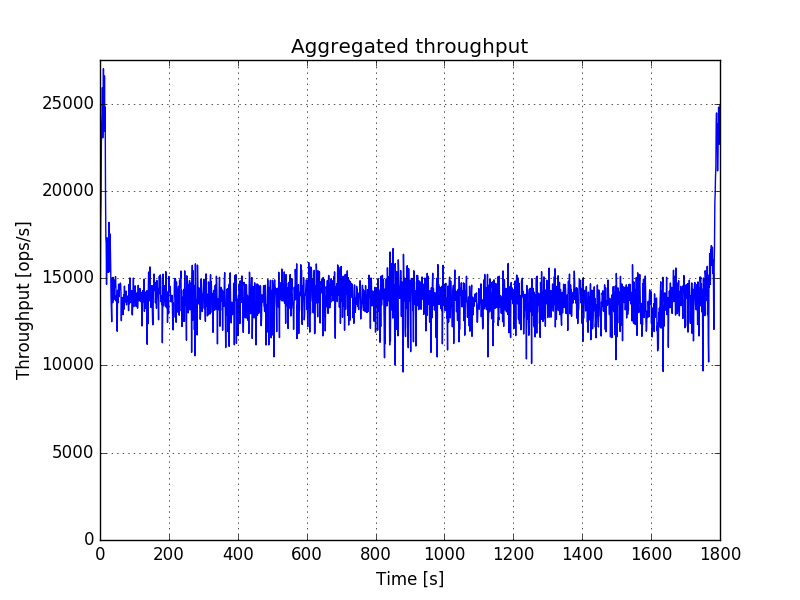
\includegraphics[width=0.95\linewidth]{plots/mm1_throughput}
\caption{Stability experiment repeated - throughput}
\label{fig:mm1-throughput}
\end{figure}

\begin{figure}
\centering
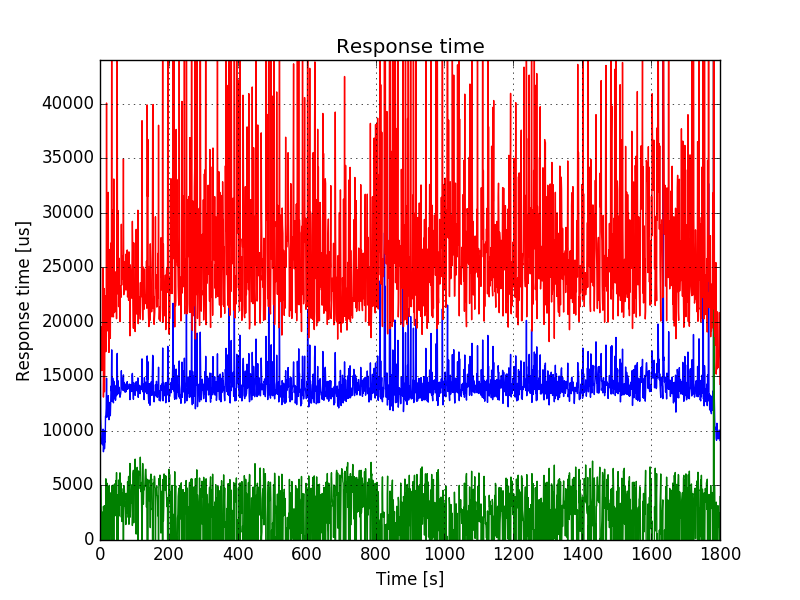
\includegraphics[width=0.95\linewidth]{plots/mm1_response_time}
\caption{Stability experiment repeated - response time}
\label{fig:mm1-response-time}
\end{figure}

\end{document}
